% id: 129-54
% book: 베이직쎈 대수 · 07 삼각함수의 그래프
% section: 개념 47 삼각방정식
% passage: 다음 방정식을 푸시오.
% figure: none
% answer: 
% answer_source: 
% variant_level: 0 (원본 전사)
% 이 파일은 build.mjs 가 items.json 에서 만든다. 고칠 때는 items.json 을 고친다.
\smash{\raisebox{4.5mm}{\dmkichul{베이직쎈 대수 129쪽 54번}}}
$\sin\left(2x-\dfrac{\pi}{4}\right)=\dfrac{\sqrt{2}}{2}$ \dmcondfill{$0\le x<\pi$}{}
\dmhint{$2x-\dfrac{\pi}{4}=\theta$로 놓으면 \quad $\blank\le\theta<\blank$\\ 주어진 방정식은 \quad $\sin\theta=\dfrac{\sqrt{2}}{2}$\par\smallskip\dispeq{% 129-54(129쪽) — 🎯 힌트 안 그래프: $\theta=2x-\frac{\pi}{4}$ 로 놓았을 때 $y=\sin\theta$ $\left(-\frac{\pi}{4}\le\theta<\frac{7}{4}\pi\right)$ 와 직선 $y=\frac{\sqrt{2}}{2}$.
% 스캔 화질이 낮아 TikZ 로 다시 그림. 라벨은 원문에 있는 것만 — $1$·$-1$, $-\frac{\pi}{4}$·$\frac{\pi}{2}$·$\pi$·$\frac{3}{2}\pi$·$\frac{7}{4}\pi$.
% 교점의 $\theta$ 값(답으로 이어지는 값)은 원문에도 없으므로 점만 찍는다. 왼쪽 끝은 닫힌 점, 오른쪽 끝은 열린 점.
\begin{tikzpicture}[line width=0.6pt, x=0.80cm, y=0.72cm]
  \draw[dotted, line width=0.5pt] (0,1) -- (1.5708,1) (1.5708,0) -- (1.5708,1);
  \draw[dotted, line width=0.5pt] (0,-1) -- (4.7124,-1) (4.7124,0) -- (4.7124,-1);
  \draw[->, >=stealth, line width=0.7pt] (-1.95,0) -- (6.55,0) node[below=1pt, font=\footnotesize] {$\theta$};
  \draw[->, >=stealth, line width=0.7pt] (0,-1.70) -- (0,1.80) node[left=1pt, font=\footnotesize] {$y$};
  \draw[line width=0.6pt] (-1.95,0.7071) -- (6.20,0.7071);
  \draw[line width=0.7pt, domain=-0.7854:5.4978, samples=140, smooth] plot (\x, {sin(57.2958*\x)});
  \fill (-0.7854,-0.7071) circle (1.7pt);
  \draw[fill=white, line width=0.5pt] (5.4978,-0.7071) circle (1.7pt);
  \fill[red!75] (0.7854,0.7071) circle (1.7pt);
  \fill[red!75] (2.3562,0.7071) circle (1.7pt);
  \node[anchor=east, font=\footnotesize] at (-0.12,1) {$1$};
  \node[anchor=east, font=\footnotesize] at (-0.12,-1) {$-1$};
  \node[anchor=south east, font=\footnotesize] at (-0.10,0.04) {$-\dfrac{\pi}{4}$};
  \node[anchor=north, font=\footnotesize] at (0.18,-0.06) {$\pt{O}$};
  \node[anchor=north, font=\footnotesize] at (1.5708,-0.10) {$\dfrac{\pi}{2}$};
  \node[anchor=south, font=\footnotesize, fill=white, inner sep=0.6pt] at (3.1416,0.05) {$\pi$};
  \node[anchor=south, font=\footnotesize, fill=white, inner sep=0.6pt] at (4.7124,0.05) {$\dfrac{3}{2}\pi$};
  \node[anchor=north west, font=\footnotesize] at (5.62,-0.30) {$\dfrac{7}{4}\pi$};
  \draw[->, >=stealth, line width=0.4pt] (5.62,-0.34) -- (5.45,-0.62);
  \node[anchor=south west, font=\footnotesize] at (1.00,1.04) {$y=\sin\theta$};
  \node[anchor=south east, font=\footnotesize] at (6.18,0.76) {$y=\dfrac{\sqrt{2}}{2}$};
\end{tikzpicture}
}\par\smallskip\noindent $\sin\theta=\dfrac{\sqrt{2}}{2}$의 해를 구하면 \quad $\theta=\blank$ 또는 $\theta=\blank[2.4em]$\\ 즉 $2x-\dfrac{\pi}{4}=\blank$ 또는 $2x-\dfrac{\pi}{4}=\blank[2.4em]$이므로\\ \hspace*{1.5em}$x=\blank$ 또는 $x=\blank$}
